\documentclass[11pt,a4paper]{report}
\usepackage[textwidth=37em,vmargin=30mm]{geometry}
\usepackage{calc,xunicode,amsmath,amssymb,paralist,enumitem,tabu,booktabs,datetime2,xeCJK,xeCJKfntef,listings}
\usepackage{tocloft,fancyhdr,tcolorbox,xcolor,graphicx,eso-pic,xltxtra,xelatexemoji}

\newcommand{\envyear}[0]{2025}
\newcommand{\envdatestr}[0]{2025-07-01}
\newcommand{\envfinaldir}[0]{webdb/2025/20250701/final}

\usepackage[hidelinks]{hyperref}
\hypersetup{
    colorlinks=false,
    pdfpagemode=FullScreen,
    pdftitle={Web Digest - \envdatestr}
}

\setlength{\cftbeforechapskip}{10pt}
\renewcommand{\cftchapfont}{\rmfamily\bfseries\large\raggedright}
\setlength{\cftbeforesecskip}{2pt}
\renewcommand{\cftsecfont}{\sffamily\small\raggedright}

\setdefaultleftmargin{2em}{2em}{1em}{1em}{1em}{1em}

\usepackage{xeCJK,xeCJKfntef}
\xeCJKsetup{PunctStyle=plain,RubberPunctSkip=false,CJKglue=\strut\hskip 0pt plus 0.1em minus 0.05em,CJKecglue=\strut\hskip 0.22em plus 0.2em}
\XeTeXlinebreaklocale "zh"
\XeTeXlinebreakskip = 0pt


\setmainfont{Brygada 1918}
\setromanfont{Brygada 1918}
\setsansfont{IBM Plex Sans}
\setmonofont{JetBrains Mono NL}
\setCJKmainfont{Noto Serif CJK SC}
\setCJKromanfont{Noto Serif CJK SC}
\setCJKsansfont{Noto Sans CJK SC}
\setCJKmonofont{Noto Sans CJK SC}

\setlength{\parindent}{0pt}
\setlength{\parskip}{8pt}
\linespread{1.15}

\lstset{
	basicstyle=\ttfamily\footnotesize,
	numbersep=5pt,
	backgroundcolor=\color{black!5},
	showspaces=false,
	showstringspaces=false,
	showtabs=false,
	tabsize=2,
	captionpos=b,
	breaklines=true,
	breakatwhitespace=true,
	breakautoindent=true,
	linewidth=\textwidth
}






\newcommand{\coverpic}[2]{
    % argv: itemurl, authorname
    Cover photo by #2~~(\href{#1}{#1})
}
\newcommand{\makeheader}[0]{
    \begin{titlepage}
        % \newgeometry{hmargin=15mm,tmargin=21mm,bmargin=12mm}
        \begin{center}
            
            \rmfamily\scshape
            \fontspec{BaskervilleF}
            \fontspec{Old Standard}
            \fontsize{59pt}{70pt}\selectfont
            WEB\hfill DIGEST
            
            \vfill
            % \vskip 30pt
            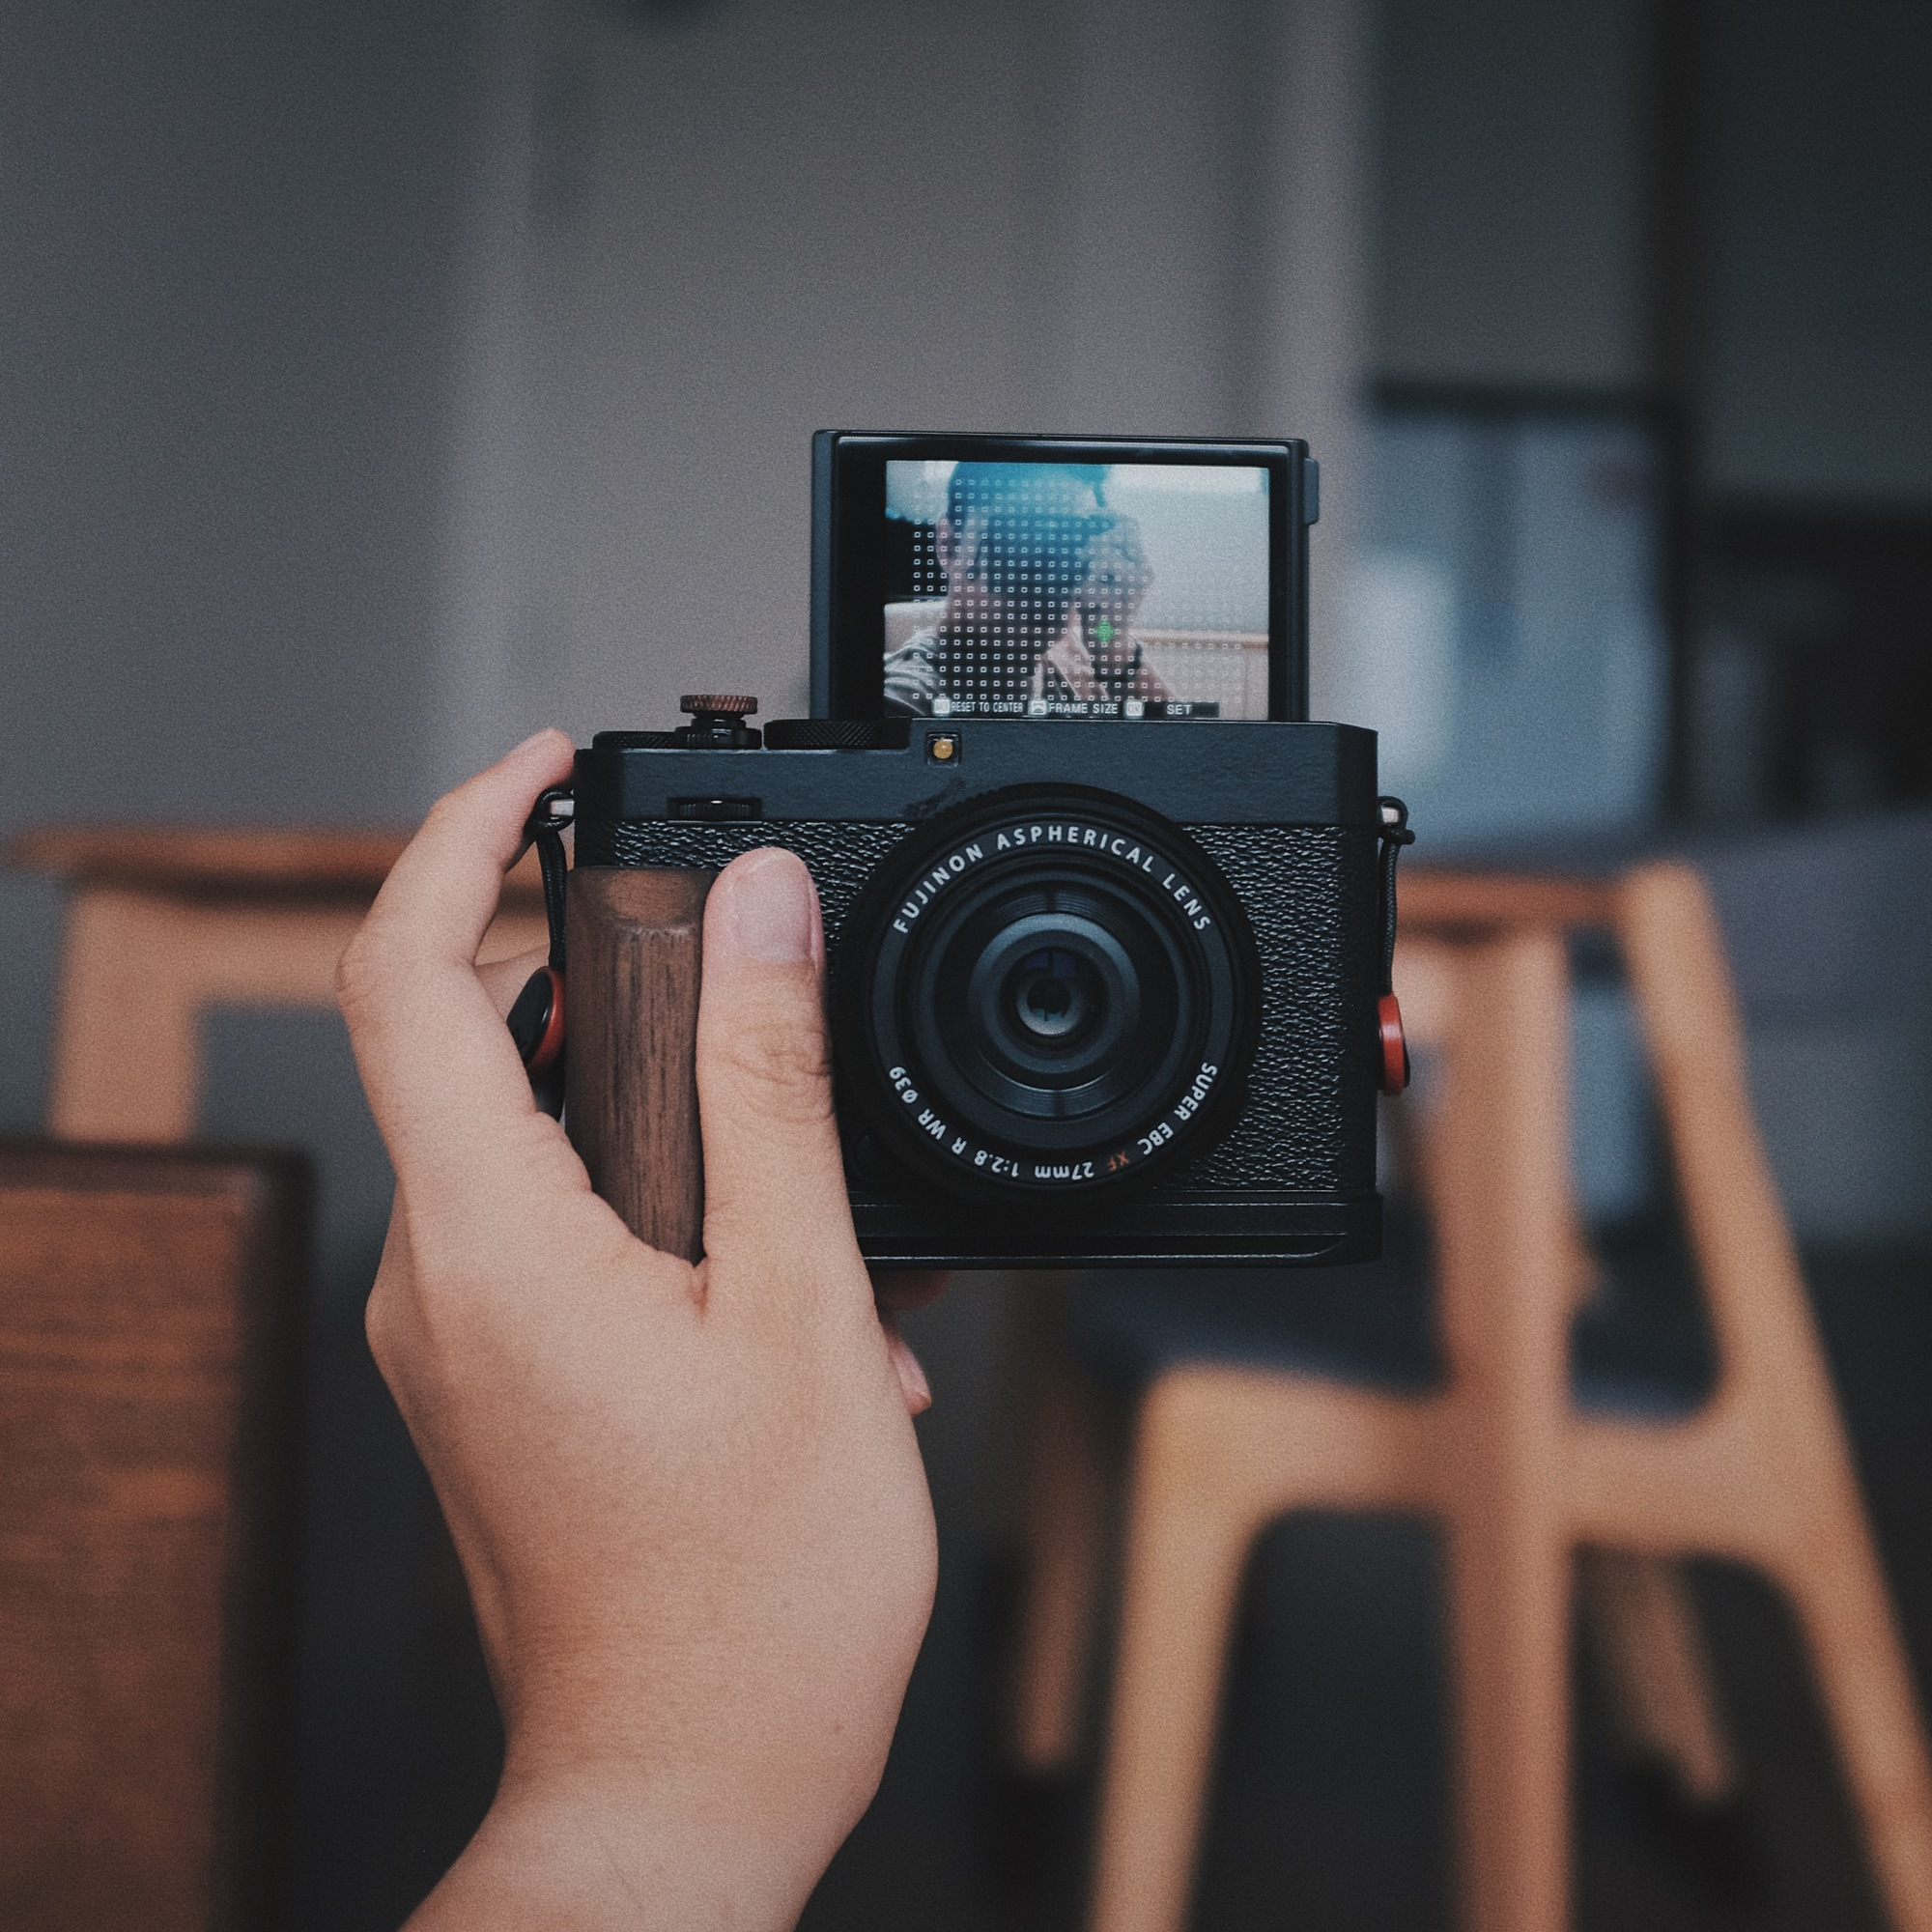
\includegraphics[width=\linewidth]{\envfinaldir/coverpic-prod.jpg}\par
            % \vskip 30pt
            \vfill

            \normalsize\rmfamily\scshape
            \copyright{} The Web Digest Project \hfill\large \envdatestr
        \end{center}
    \end{titlepage}
    % \restoregeometry
}
\newcommand{\simplehref}[1]{%
    \textcolor{blue!80!green}{\href{#1}{#1}}%
}
\renewcommand{\contentsname}{\center\Huge\sffamily\bfseries Contents\par\vskip 20pt}
\newcounter{ipartcounter}
\setcounter{ipartcounter}{0}
\newcommand{\ipart}[1]{
    % \vskip 20pt
    \clearpage
    \stepcounter{ipartcounter}
    \phantomsection
    \addcontentsline{toc}{chapter}{#1}
    % \begin{center}
    %     \Huge
    %     \sffamily\bfseries
    %     #1
    % \end{center}
    % \vskip 20pt plus 7pt
}
\newcounter{ichaptercounter}
\setcounter{ichaptercounter}{0}
\newcommand{\ichapter}[1]{
    % \vskip 20pt
    \clearpage
    \stepcounter{ichaptercounter}
    \phantomsection
    \addcontentsline{toc}{section}{\numberline{\arabic{ichaptercounter}}#1}
    \begin{center}
        \Huge
        \sffamily\bfseries
        #1
    \end{center}
    \vskip 20pt plus 7pt
}
\newcommand{\entrytitlefont}[1]{\subsection*{\raggedright\Large\sffamily\bfseries#1}}
\newcommand{\entryitemGeneric}[2]{
    % argv: title, url
    \parbox{\linewidth}{
        \entrytitlefont{#1}\par\vskip 5pt
        \footnotesize\ttfamily\mdseries
        \simplehref{#2}
    }\vskip 11pt plus 11pt minus 1pt
}
\newcommand{\entryitemGithub}[3]{
    % argv: title, url, desc
    \parbox{\linewidth}{
        \entrytitlefont{#1}\par\vskip 5pt
        \footnotesize\ttfamily\mdseries
        \simplehref{#2}\par\vskip 5pt
        \small\rmfamily\mdseries#3
    }\vskip 11pt plus 11pt minus 1pt
}
\newcommand{\entryitemAp}[3]{
    % argv: title, url, desc
    \parbox{\linewidth}{
        \entrytitlefont{#1}\par\vskip 5pt
        \footnotesize\ttfamily\mdseries
        \simplehref{#2}\par\vskip 5pt
        \small\rmfamily\mdseries#3
    }\vskip 11pt plus 11pt minus 1pt
}
\newcommand{\entryitemHackernews}[3]{
    % argv: title, hnurl, rawurl
    % \parbox{\linewidth}{
    %     \entrytitlefont{#1}\par\vskip 5pt
    %     \footnotesize\ttfamily\mdseries
    %     \simplehref{#3}\par
    %     \textcolor{black!50}{\href{#2}{#2}}
    % }\vskip 11pt plus 11pt minus 1pt
    \begin{minipage}{\linewidth}
            \entrytitlefont{#1}\par\vskip 5pt
            \footnotesize\ttfamily\mdseries
            \simplehref{#3}\par
            \textcolor{black!50}{\href{#2}{#2}}
    \end{minipage}\par\vskip 11pt plus 11pt minus 1pt
}







\begin{document}

\makeheader

\tableofcontents\clearpage




\ipart{Developers}
\ichapter{Hacker News}
\entryitemTwoLinks{The New Skill in AI Is Not Prompting, It's Context Engineering}{https://news.ycombinator.com/item?id=44427757}{https://www.philschmid.de/context-engineering}

\entryitemTwoLinks{Xfinity using WiFi signals in your house to detect motion}{https://news.ycombinator.com/item?id=44426726}{https://www.xfinity.com/support/articles/wifi-motion}

\entryitemTwoLinks{The hidden JTAG in a Qualcomm/Snapdragon device's USB port}{https://news.ycombinator.com/item?id=44426428}{https://www.linaro.org/blog/hidden-jtag-qualcomm-snapdragon-usb/}

\entryitemTwoLinks{Datadog's \$65M/year customer mystery solved}{https://news.ycombinator.com/item?id=44426399}{https://blog.pragmaticengineer.com/datadog-65m-year-customer-mystery/}

\entryitemTwoLinks{Ask HN: What's the 2025 stack for a self-hosted photo library with local AI?}{https://news.ycombinator.com/item?id=44426233}{https://news.ycombinator.com/item?id=44426233}

\entryitemTwoLinks{Proton joins suit against Apple for predatory practices}{https://news.ycombinator.com/item?id=44426128}{https://proton.me/blog/apple-lawsuit}

\entryitemTwoLinks{I write type-safe generic data structures in C}{https://news.ycombinator.com/item?id=44425461}{https://danielchasehooper.com/posts/typechecked-generic-c-data-structures/}

\entryitemTwoLinks{Donkey Kong Country 2 and Open Bus}{https://news.ycombinator.com/item?id=44424194}{https://jsgroth.dev/blog/posts/dkc2-open-bus/}

\entryitemTwoLinks{There are no new ideas in AI only new datasets}{https://news.ycombinator.com/item?id=44423983}{https://blog.jxmo.io/p/there-are-no-new-ideas-in-ai-only}

\entryitemTwoLinks{Show HN: TokenDagger – A tokenizer faster than OpenAI's Tiktoken}{https://news.ycombinator.com/item?id=44422480}{https://github.com/M4THYOU/TokenDagger}

\entryitemTwoLinks{Entry-level jobs down by a third since launch of ChatGPT}{https://news.ycombinator.com/item?id=44422040}{https://www.personneltoday.com/hr/fall-in-entry-level-jobs-linked-to-rise-of-ai-tools/}

\entryitemTwoLinks{Show HN: New Ensō – first public beta}{https://news.ycombinator.com/item?id=44421776}{https://untested.sonnet.io/notes/new-enso-first-public-beta/}

\entryitemTwoLinks{The provenance memory model for C}{https://news.ycombinator.com/item?id=44421185}{https://gustedt.wordpress.com/2025/06/30/the-provenance-memory-model-for-c/}

\entryitemTwoLinks{Want to meet people, try charging them for it?}{https://news.ycombinator.com/item?id=44419986}{https://notes.eatonphil.com/2025-06-28-want-to-meet-people-charge-them.html}

\entryitemTwoLinks{LetsEncrypt – Expiration Notification Service Has Ended}{https://news.ycombinator.com/item?id=44419496}{https://letsencrypt.org/2025/06/26/expiration-notification-service-has-ended/}

\entryitemTwoLinks{Bought myself an Ampere Altra system}{https://news.ycombinator.com/item?id=44419446}{https://marcin.juszkiewicz.com.pl/2025/06/27/bought-myself-an-ampere-altra-system/}

\entryitemTwoLinks{Gridfinity: The modular, open-source grid storage system}{https://news.ycombinator.com/item?id=44419091}{https://gridfinity.xyz/}

\entryitemTwoLinks{The Chan-Zuckerbergs stopped funding social causes}{https://news.ycombinator.com/item?id=44418105}{https://www.washingtonpost.com/technology/2025/06/29/mark-zuckerberg-priscilla-chan-school-closure/}

\entryitemTwoLinks{Nearly 20\% of cancer drugs defective in four African nations}{https://news.ycombinator.com/item?id=44417549}{https://www.dw.com/en/nearly-20-of-cancer-drugs-defective-in-4-african-nations/a-73062221}

\entryitemTwoLinks{ICE test train reaches speeds of up to 405.0 km/h}{https://news.ycombinator.com/item?id=44417276}{https://www.deutschebahn.com/de/presse/pressestart\_zentrales\_uebersicht/ICE-Testzug-faehrt-bis-zu-405-0-km-h-und-sammelt-wichtige-Erkenntnisse-fuer-den-Hochgeschwindigkeitsverkehr-13428394}


\ipart{Developers~~~~(zh-Hans)}
\ichapter{Solidot}
\entryitemGeneric{\hskip 0pt{}小行星 2024 YR4 撞击月球概率上升至 1/25}{https://www.solidot.org/story?sid=81679}

\entryitemGeneric{\hskip 0pt{}碳记录显示人类五万年前开始大规模用火}{https://www.solidot.org/story?sid=81678}

\entryitemGeneric{\hskip 0pt{}研究发现消费者对 AI 产品信任度低}{https://www.solidot.org/story?sid=81677}

\entryitemGeneric{\hskip 0pt{}Canonical 2024 年营收 2.92 亿美元}{https://www.solidot.org/story?sid=81676}

\entryitemGeneric{\hskip 0pt{}研究发现白垩纪海洋是``乌贼的天下''}{https://www.solidot.org/story?sid=81675}

\entryitemGeneric{\hskip 0pt{}日本争议夫妇别姓法案}{https://www.solidot.org/story?sid=81674}

\entryitemGeneric{\hskip 0pt{}中国平面设计师面临 AI 图像生成器的挑战}{https://www.solidot.org/story?sid=81673}

\entryitemGeneric{\hskip 0pt{}Bcachefs 文件系统可能将会移除出内核}{https://www.solidot.org/story?sid=81672}

\entryitemGeneric{\hskip 0pt{}德国要求苹果和 Google 下架 DeepSeek}{https://www.solidot.org/story?sid=81671}\ichapter{V2EX}
\entryitemGeneric{\hskip 0pt{}[分享发现] 有毛被洗的桃子请慎重选购}{https://www.v2ex.com/t/1142112}

\entryitemGeneric{\hskip 0pt{}[程序员] 有篇 2021 年的文章说 epoll 早于 kqueue,我的同事差点被误导}{https://www.v2ex.com/t/1142106}

\entryitemGeneric{\hskip 0pt{}[推广] 专业图床欢迎使用}{https://www.v2ex.com/t/1142105}

\entryitemGeneric{\hskip 0pt{}[生活] iPad 上的 YouTube 好糊啊}{https://www.v2ex.com/t/1142104}

\entryitemGeneric{\hskip 0pt{}[生活] 咨询一下大家关于孕期检查的问题}{https://www.v2ex.com/t/1142103}

\entryitemGeneric{\hskip 0pt{}[Apple] 我终于找到了 Apple 自带输入法不好用的根本原因}{https://www.v2ex.com/t/1142102}

\entryitemGeneric{\hskip 0pt{}[问与答] 喜报: 港版三星钱包 支持 NFC 门禁了 (限 android 15)}{https://www.v2ex.com/t/1142101}

\entryitemGeneric{\hskip 0pt{}[酷工作] 招全职远程安卓开发工程师(需同时有 IOS 开发经验),月薪 3500 美金}{https://www.v2ex.com/t/1142099}

\entryitemGeneric{\hskip 0pt{}[分享创造] MySQL 語法兼容的 WASM 實現}{https://www.v2ex.com/t/1142098}

\entryitemGeneric{\hskip 0pt{}[问与答] ibkr 有存款保险吗}{https://www.v2ex.com/t/1142097}

\entryitemGeneric{\hskip 0pt{}[Java] 胡思乱想(针对企业的 ai 平台应用)}{https://www.v2ex.com/t/1142096}

\entryitemGeneric{\hskip 0pt{}[问与答] 咨询大家关于孕期检查的问题}{https://www.v2ex.com/t/1142095}

\entryitemGeneric{\hskip 0pt{}[程序员] 看到一些 github 项目作者,总是千方百计利诱网友给予 star}{https://www.v2ex.com/t/1142094}

\entryitemGeneric{\hskip 0pt{}[程序员] Dokploy 用了一段时间,确实好使}{https://www.v2ex.com/t/1142093}

\entryitemGeneric{\hskip 0pt{}[硬件] 无屏幕的 AI 眼镜,为啥不做成耳机?}{https://www.v2ex.com/t/1142091}

\entryitemGeneric{\hskip 0pt{}[分享发现] 中医治好了我}{https://www.v2ex.com/t/1142089}

\entryitemGeneric{\hskip 0pt{}[OpenAI] 🎁免费的 GPT-4.1 min 模型 API,可用于沉浸式翻译}{https://www.v2ex.com/t/1142088}

\entryitemGeneric{\hskip 0pt{}[分享发现] 一个有意思的工具 https://www.playphrase.me/}{https://www.v2ex.com/t/1142087}

\entryitemGeneric{\hskip 0pt{}[问与答] 大家的广电卡有没有感觉网页加载速度慢?}{https://www.v2ex.com/t/1142086}

\entryitemGeneric{\hskip 0pt{}[问与答] ios 上订阅 Claude code max 版 5x 和 20x,怎么比网页贵这么多吗?价格是 124.99 刀和 249.99 刀}{https://www.v2ex.com/t/1142085}

\entryitemGeneric{\hskip 0pt{}[macOS] Mac 上的微信双开方法}{https://www.v2ex.com/t/1142084}

\entryitemGeneric{\hskip 0pt{}[生活] 男 V 友相亲的时候有和对方 AA 过吗?}{https://www.v2ex.com/t/1142083}

\entryitemGeneric{\hskip 0pt{}[程序员] QQ 新版感觉太臃肿, Tim 有听说会扫盘}{https://www.v2ex.com/t/1142082}

\entryitemGeneric{\hskip 0pt{}[问与答] 买了一个 6 元的手机壳,还包邮,这些商家是咋赚钱的}{https://www.v2ex.com/t/1142081}

\entryitemGeneric{\hskip 0pt{}[问与答] 我这个鼠标垫在湿度大时感觉非常不爽}{https://www.v2ex.com/t/1142080}

\entryitemGeneric{\hskip 0pt{}[Apple] iPhone 15 pro 空气充电}{https://www.v2ex.com/t/1142079}

\entryitemGeneric{\hskip 0pt{}[分享发现] 键盘老人机+电信偷跑流量,话费暴涨}{https://www.v2ex.com/t/1142077}

\entryitemGeneric{\hskip 0pt{}[分享创造] 周末临时起意 vibe coding 了一个纯粹的在线拼图工具}{https://www.v2ex.com/t/1142076}

\entryitemGeneric{\hskip 0pt{}[NAS] 请教各位佬一个 moviepilot 的问题}{https://www.v2ex.com/t/1142075}

\entryitemGeneric{\hskip 0pt{}[优惠信息] 大润发每月 4 次 100 减 20,持续一年}{https://www.v2ex.com/t/1142074}

\entryitemGeneric{\hskip 0pt{}[MySQL] 跨平台的 MySQL Parser}{https://www.v2ex.com/t/1142073}

\entryitemGeneric{\hskip 0pt{}[远程工作] [远程] PHP 全栈和 Java 远程岗位招聘}{https://www.v2ex.com/t/1142072}

\entryitemGeneric{\hskip 0pt{}[问与答] tvOS 版 Loon 是否支持旁路由功能}{https://www.v2ex.com/t/1142071}

\entryitemGeneric{\hskip 0pt{}[Apple] jetbrains toolbox 里面下载的 app 无法通过 spotlight 进行搜索怎么办}{https://www.v2ex.com/t/1142069}

\entryitemGeneric{\hskip 0pt{}[macOS] 卸载深信服零信任客户端 atrust 遇到困惑 为什么资源库里面相关的文件移到废纸篓之后无法清空}{https://www.v2ex.com/t/1142068}

\entryitemGeneric{\hskip 0pt{}[分享发现] (新活动)华为云 1 元考证换代金券活动开始啦。}{https://www.v2ex.com/t/1142067}

\entryitemGeneric{\hskip 0pt{}[程序员] clash 开了系统代理以后,所有和微软有关的服务都登录不了, edge 账号登陆、Vscode 同步等,有需要什么特别设置的吗?}{https://www.v2ex.com/t/1142066}

\entryitemGeneric{\hskip 0pt{}[酷工作] 外企 Kong 中国研发中心搭建 3 年多啦,还在持续扩张中,接下来还有将近 20 个核心开发岗位对外招聘哦!}{https://www.v2ex.com/t/1142065}

\entryitemGeneric{\hskip 0pt{}[云计算] 关于轻量服务器以及 cdn 采购的一些问题}{https://www.v2ex.com/t/1142064}

\entryitemGeneric{\hskip 0pt{}[问与答] 有什么好的防蚊防虫方法吗?}{https://www.v2ex.com/t/1142063}

\entryitemGeneric{\hskip 0pt{}[生活] 烦恼:我有 5 块 2.5 寸 1T 的移动机械硬盘、2 块 1T 的移动固态硬盘、2 块 2T 的移动固态硬盘但是没有 1 块 16T 的机械硬盘}{https://www.v2ex.com/t/1142062}

\entryitemGeneric{\hskip 0pt{}[电影] 重温了下葫芦娃 发现还是很好看}{https://www.v2ex.com/t/1142060}

\entryitemGeneric{\hskip 0pt{}[分享创造] 钛盘 - 简单好用的文件分享服务}{https://www.v2ex.com/t/1142059}

\entryitemGeneric{\hskip 0pt{}[程序员] 有必要在 bug 上开发新功能吗}{https://www.v2ex.com/t/1142058}

\entryitemGeneric{\hskip 0pt{}[职场话题] 招聘贴 北京-招聘测试、AI 产品经理、 Java 研发、算法岗}{https://www.v2ex.com/t/1142057}

\entryitemGeneric{\hskip 0pt{}[Chrome] Chrome 的这个 profile 崩溃问题有解决方法吗?}{https://www.v2ex.com/t/1142056}

\entryitemGeneric{\hskip 0pt{}[问与答] 有没有对标 Sunfire 的开源日志监控系统}{https://www.v2ex.com/t/1142055}

\entryitemGeneric{\hskip 0pt{}[分享创造] 开发了一个把 Arc 浏览器 UI 带到 Chrome 的插件}{https://www.v2ex.com/t/1142053}

\entryitemGeneric{\hskip 0pt{}[Chrome] 求助, Chrome 浏览器在我这挂壁了?}{https://www.v2ex.com/t/1142050}

\entryitemGeneric{\hskip 0pt{}[问与答] Linux 系统笔记本纯电池待机时间太短,如何解决}{https://www.v2ex.com/t/1142048}


\ipart{Generic News}







\clearpage
\leavevmode\vfill
\footnotesize

Copyright \copyright{} 2023-2025 Neruthes and other contributors.

This document is published with CC BY-NC-ND 4.0 license.

The entries listed in this newsletter may be copyrighted by their respective creators.

This newsletter is generated by the Web Digest project.

The newsletters are also delivered via Telegram channel \CJKunderline{\href{https://t.me/webdigestchannel}{https://t.me/webdigestchannel}}.\\
RSS feed is available at \CJKunderline{\href{https://webdigest.pages.dev/rss.xml}{https://webdigest.pages.dev/rss.xml}}.

This newsletter is available in PDF at
\CJKunderline{\href{https://webdigest.pages.dev/}{https://webdigest.pages.dev/}}.

The source code being used to generate this newsletter is available at\\
\CJKunderline{\href{https://github.com/neruthes/webdigest}{https://github.com/neruthes/webdigest}}.

This newsletter is also available in
\CJKunderline{\href{http://webdigest.pages.dev/readhtml/\envyear/WebDigest-20250701.html}{HTML}} and
\CJKunderline{\href{https://github.com/neruthes/webdigest/blob/master/markdown/\envyear/WebDigest-20250701.md}{Markdown}}.


\coverpic{https://unsplash.com/photos/a-sleek-blurred-car-speeds-through-a-tunnel-8\_Ar9WZFEcg}{Luke Miller}


\end{document}
